\PassOptionsToPackage{table,dvipsnames}{xcolor}
\documentclass[
  xcolor={table,dvipsnames},
  10pt,
  aspectratio=169,
]{beamer}
\usepackage[utf8]{inputenc}
\usepackage[T1]{fontenc}
\usepackage[english]{babel}

\usetheme{ru}

\usepackage{appendixnumberbeamer}
\usepackage{microtype}
\usepackage{booktabs}
\usepackage{tabularx}
\usepackage[scale=2]{ccicons}
\usepackage{graphicx}
\usepackage{caption}
\usepackage{wrapfig}
\usepackage{bbding}

\usepackage{pgfplots}
\usepgfplotslibrary{dateplot}

\usepackage{amsmath,mathtools}

\usepackage{xspace}

\usepackage{listings}
\usepackage{lstjasmin}

\usepackage{tikz}
\usetikzlibrary{overlay-beamer-styles}
\usetikzlibrary{positioning}

\definecolor{beamer@asblue}{rgb}{.0429,.1718,.4726}
\definecolor{myred}{RGB}{194,48,27}
\newcommand{\rd}{\color{myred}}

\newcommand{\NTT}{\mbox{\textsf{NTT}}\xspace}
\newcommand{\INVNTT}{\ensuremath{\mbox{\textsf{NTT}}^{-1}}\xspace}

\newcommand{\pw}{\circ}

\newcommand{\Z}{\mathbb{Z}}
\newcommand{\F}{\mathbb{F}}

\newcommand{\pk}{\mathit{pk}}
\newcommand{\sk}{\mathit{sk}}

\newcommand{\MS}{\mathcal{M}}
\newcommand{\KS}{\mathcal{K}}
\newcommand{\RO}{\text{H}}
\newcommand{\ROH}{\text{H}}
\newcommand{\ROG}{\text{G}}
\newcommand{\PRF}{\text{PRF}}
\newcommand{\KDF}{\text{KDF}}
\newcommand{\cat}{\ensuremath{\Vert}}


\newcommand{\KEM}{\mathsf{KEM}}
\newcommand{\KEMGen}{\mathsf{KeyGen}}
\newcommand{\KEMEnc}{\mathsf{Encaps}}
%\newcommand{\PKEEncO}{\procfont{Enc}}
%\newcommand{\PKEDecO}{\procfont{Dec}}
\newcommand{\KEMDecO}{\textsc{Decaps}}
\newcommand{\KEMDec}{\mathsf{Decaps}}
\newcommand{\AdvKEMcca}[2]{\Adv^{\cca}_{#1}(#2)}

\newcommand{\A}{\mathsf{A}}
\newcommand{\B}{\mathsf{B}}
\newcommand{\PKE}{\mathsf{PKE}}
\newcommand{\PKEGen}{\mathsf{KeyGen}}
\newcommand{\PKEEnc}{\mathsf{Enc}}
\newcommand{\PKEDecO}{\textsc{Dec}}
\newcommand{\PKEDec}{\mathsf{Dec}}
\newcommand{\Kyber}{\ensuremath{\mathsf{Kyber}}}
\newcommand{\KyberCPA}{\ensuremath{\mathsf{Kyber.CPA}}}
\newcommand{\KyberCPAd}{\ensuremath{\mathsf{Kyber.CPA.det}}}
\newcommand{\KyberHybrid}{\ensuremath{\mathsf{Kyber.Hybrid}}}
\newcommand{\KyberUAKE}{\ensuremath{\mathsf{Kyber.UAKE}}}
\newcommand{\KyberAKE}{\ensuremath{\mathsf{Kyber.AKE}}}
\newcommand{\KyberKE}{\ensuremath{\mathsf{Kyber.KE}}}
\newcommand{\XOF}{\ensuremath{\mathsf{XOF}}}
\newcommand{\prefix}{\ensuremath{\mathsf{prefix}}}
\newcommand{\mlkem}{\text{{ML-KEM}}\xspace}
\newcommand{\mlkemMid}{\sc ML-KEM-768\xspace}
\newcommand{\mldsa}{\text{{ML-DSA}}\xspace}
\newcommand{\slhdsa}{\text{{SLH-DSA}}\xspace}

\newcommand{\KyberCompress}{\ensuremath{\mathsf{Compress}}\xspace}
\newcommand{\KyberDecompress}{\ensuremath{\mathsf{Decompress}}\xspace}

\newcommand{\xpo}{\mathbf{x}}
\newcommand{\ypo}{\mathbf{y}}
\newcommand{\cpo}{\mathbf{c}}
\newcommand{\vpo}{\mathbf{v}}
\newcommand{\Apo}{\mathbf{A}}
\newcommand{\epo}{\mathbf{e}}
\newcommand{\spo}{\mathbf{s}}
\newcommand{\tpo}{\mathbf{t}}
\newcommand{\rpo}{\mathbf{r}}
\newcommand{\wpo}{\mathbf{w}}
\newcommand{\upo}{\mathbf{u}}
\newcommand{\dpo}{\mathbf{d}}
\newcommand{\gpo}{\mathbf{g}}
\newcommand{\fpo}{\mathbf{f}}
\newcommand{\zpo}{\mathbf{z}}

\newcommand{\apo}{\mathbf{a}}
\newcommand{\bpo}{\mathbf{b}}

\newcommand{\Sam}{\mathsf{Sam}}

\newcommand{\KyberLow}{{\sc Kyber}512\xspace}
\newcommand{\KyberMid}{{\sc Kyber}768\xspace}
\newcommand{\KyberHigh}{{\sc Kyber}1024\xspace}


%MACROS for performance
\newcommand{\LowSKBytes}{$1632$}
\newcommand{\LowPKBytes}{$800$}
\newcommand{\LowCTBytes}{$736$}
\newcommand{\LowGenCyclesAVX}{$29100$}
\newcommand{\LowEncCyclesAVX}{$46196$}
\newcommand{\LowDecCyclesAVX}{$39410$}
\newcommand{\LowGenStack}{$XXX$}
\newcommand{\LowEncStack}{$XXX$}
\newcommand{\LowDecStack}{$XXX$}
\newcommand{\LowGenCyclesARM}{$XXX$}
\newcommand{\LowEncCyclesARM}{$XXX$}
\newcommand{\LowDecCyclesARM}{$XXX$}
\newcommand{\LowGenCyclesN}{$15792$}
\newcommand{\LowEncCyclesN}{$26612$}
\newcommand{\LowDecCyclesN}{$22248$}

\newcommand{\MidSKBytes}{$2400$}
\newcommand{\MidPKBytes}{$1184$}
\newcommand{\MidCTBytes}{$1088$}
\newcommand{\MidGenCyclesAVX}{$57340$}
\newcommand{\MidEncCyclesAVX}{$78692$}
\newcommand{\MidDecCyclesAVX}{$68620$}
\newcommand{\MidGenStack}{$XXX$}
\newcommand{\MidEncStack}{$XXX$}
\newcommand{\MidDecStack}{$XXX$}
\newcommand{\MidGenCyclesARM}{$XXX$}
\newcommand{\MidEncCyclesARM}{$XXX$}
\newcommand{\MidDecCyclesARM}{$XXX$}
\newcommand{\MidGenCyclesN}{$25632$}
\newcommand{\MidEncCyclesN}{$39976$}
\newcommand{\MidDecCyclesN}{$33744$}

\newcommand{\HighSKBytes}{$3168$}
\newcommand{\HighPKBytes}{$1568$}
\newcommand{\HighCTBytes}{$1568$}
\newcommand{\HighGenCyclesAVX}{$81244$}
\newcommand{\HighEncCyclesAVX}{$109584$}
\newcommand{\HighDecCyclesAVX}{$97280$}
\newcommand{\HighGenStack}{$XXX$}
\newcommand{\HighEncStack}{$XXX$}
\newcommand{\HighDecStack}{$XXX$}
\newcommand{\HighGenCyclesARM}{$XXX$}
\newcommand{\HighEncCyclesARM}{$XXX$}
\newcommand{\HighDecCyclesARM}{$XXX$}
\newcommand{\HighGenCyclesN}{$38164$}
\newcommand{\HighEncCyclesN}{$57280$}
\newcommand{\HighDecCyclesN}{$50360$}

\newcommand{\bEasyCrypt}{\textbf{\textsc{EasyCrypt}}\xspace}
\newcommand{\EasyCrypt}{{\sc EasyCrypt}\xspace}
\newcommand{\kyber}{\text{{\sc Kyber}}\xspace}
\newcommand{\kybermid}{\kyber-768\xspace}
\newcommand{\CRYSTALSKyber}{CRYSTALS-Kyber\xspace}


\newcommand*{\loc}[1]{\tikz[remember picture]{\node [] (#1) {}}}

\title{Jasmin: high-assurance high-speed cryptography}
\author{Miguel Quaresma \and Santiago Arranz Olmos}
\institute{Max Planck Institute for Security and Privacy}
\date{September 4, 2024}

\begin{document}

\maketitle

\begin{frame}[fragile]{Efficient, correct, safe, and secure}
\begin{minipage}{0.55\linewidth}
  \lstset{
    language=Jasmin,
    basicstyle=\footnotesize\ttfamily,
    escapechar=~~,
  }
  \begin{lstlisting}
fn memeq(reg u64 p q n) -> reg u64 {~~\loc{a00}~~
  reg u64 r one i;~~\loc{a01}~~
  r = 0;~~\loc{a02}~~
  one = 1;~~\loc{a03}~~
  i = 0;~~\loc{a04}~~
  while (i < n) {~~\loc{a05}~~
    if (r != 0) {~~\loc{a06}~~
      reg u64 a b;
      a = [p];~~\loc{a07}~~
      b = [q];~~\loc{a08}~~
      r = a != b ? one : r;~~\loc{a09}~~
      p += 8;~~\loc{a10}~~
      q += 8;~~\loc{a11}~~
    }~~\loc{a12}~~
    i = #INC(i);~~\loc{a13}~~
  }~~\loc{a14}~~
  return r;~~\loc{a15}~~
}~~\loc{a16}~~
  \end{lstlisting}
\end{minipage}\hfill%
\begin{minipage}{0.4\linewidth}
  \begin{uncoverenv}<2->
    \lstset{
      basicstyle=\scriptsize\ttfamily,
      escapechar=~~,
    }
    \begin{lstlisting}
~~\loc{b00}~~memeq:
  ~~\loc{b01}~~movq $0, %rax
  ~~\loc{b02}~~movq $1, %rcx
  ~~\loc{b03}~~movq $0, %r8
  ~~\loc{b04}~~jmp Lmemeq$1
~~\loc{b05}~~Lmemeq$2:
  ~~\loc{b06}~~cmpq $0, %rax
  ~~\loc{b07}~~je Lmemeq$3
  ~~\loc{b08}~~movq (%rdi), %r9
  ~~\loc{b09}~~movq (%rsi), %r10
  ~~\loc{b10}~~cmpq %r10, %r9
  ~~\loc{b11}~~cmovne %rcx, %rax
  ~~\loc{b12}~~addq $8, %rdi
  ~~\loc{b13}~~addq $8, %rsi
~~\loc{b14}~~Lmemeq$3:
  ~~\loc{b15}~~incq %r8
~~\loc{b16}~~Lmemeq$1:
  ~~\loc{b17}~~cmpq %rdx, %r8
  ~~\loc{b18}~~jb Lmemeq$2
  ~~\loc{b19}~~ret
    \end{lstlisting}
  \end{uncoverenv}
\end{minipage}

\begin{tikzpicture}[overlay, remember picture]
  \draw [->, visible on=<2-3>] (a02) -- (b01);
  \draw [->, visible on=<2-3>] (a03) -- (b02);
  \draw [->, visible on=<2-3>] (a04) -- (b03);
  \draw [->, visible on=<2-3>] (a07) -- (b08);
  \draw [->, visible on=<2-3>] (a08) -- (b09);
  \draw [->, visible on=<2-3>] (a09) -- (b10);
  \draw [->, visible on=<2-3>] (a09) -- (b11);
  \draw [->, visible on=<2-3>] (a10) -- (b12);
  \draw [->, visible on=<2-3>] (a11) -- (b13);
  \draw [->, visible on=<2>] (a13) -- (b15);

  \draw [->, dashed, Red, thick, visible on=<3>] (a13) -- (b15);

  \draw [->, densely dotted, thick, Green, visible on=<4>] (a00) -- (b00);
  \draw [->, densely dotted, thick, Green, visible on=<4>] (a15) -- (b19);

  \draw [->, Red, visible on=<4>] (a05) -- (b04);
  \draw [->, Red, visible on=<4>] (a05) -- (b05);
  \draw [->, Red, visible on=<4>] (a05) -- (b16);
  \draw [->, Red, visible on=<4>] (a05) -- (b17);
  \draw [->, Red, visible on=<4>] (a05) -- (b18);

  \draw [->, dashed, Blue, visible on=<4>] (a06) -- (b06);
  \draw [->, dashed, Blue, visible on=<4>] (a06) -- (b07);
  \draw [->, dashed, Blue, visible on=<4>] (a06) -- (b14);
\end{tikzpicture}%
\end{frame}


\begin{frame}{Correctness, safety, side channels}
  \begin{minipage}[t]{0.45\linewidth}
    \begin{center}
      \large{\textbf{Correctness}}
    \end{center}
    Use EasyCrypt to ensure:
    \begin{itemize}
    \item Implementation matches specification
    \item Specification is secure
    \end{itemize}
  \end{minipage} \hfill%
  \begin{minipage}[t]{0.45\linewidth}
    \uncover<2->{
      \begin{center}
        \large{\textbf{Safety}}
      \end{center}
      \begin{itemize}
      \item Termination
      \item Array accesses in bounds
      \item Arithmetic errors
      \end{itemize}
    }
  \end{minipage}


  \vspace{3em}

  \begin{minipage}[t]{0.45\linewidth}
    \uncover<3->{
      \begin{center}
        \large{\textbf{Constant time}}
      \end{center}
      runtime does not depend on\\secrets
      \begin{itemize}
      \item Control flow
      \item Memory accesses
    \end{itemize}}
  \end{minipage}\hfill%
  \begin{minipage}[t]{0.45\linewidth}
    \uncover<4>{
      \begin{center}
        \large{\textbf{Speculative constant time}}
      \end{center}
      CT even under speculative\\execution
    }
  \end{minipage}
\end{frame}


\begin{frame}[fragile]{Safety - uninitialized values}
  \lstset{
    language=Jasmin,
    basicstyle=\footnotesize\ttfamily,
    escapechar=~~,
  }
  \begin{lstlisting}
    export
    fn uninitialized() -> reg u64 {
      reg u64 x;
      x = x + 1; // Uninitialized read from x.
      return x;
    }
  \end{lstlisting}
\end{frame}

\begin{frame}[fragile]{Safety - division by zero}
  \lstset{
    language=Jasmin,
    basicstyle=\footnotesize\ttfamily,
    escapechar=~~,
  }
  \begin{lstlisting}
    export
    fn arithmetic(reg u64 x y) -> reg u64 {
      x = x / y; // y could be zero.
      return x;

    }
  \end{lstlisting}
\end{frame}


\begin{frame}[fragile]{Safety - out of bounds access}
  \lstset{
    language=Jasmin,
    basicstyle=\footnotesize\ttfamily,
    escapechar=~~
  }
  \begin{lstlisting}
    export
    fn index(reg u64 x) -> reg u64 {
      stack u64[1] s;
      s[x] = 0; // x could be out of bounds.
      x = s[0]; // s[0] could be uninitialized
      return x;
    }
  \end{lstlisting}
\end{frame}

\begin{frame}[fragile]{Safety - termination}
  \lstset{
    language=Jasmin,
    basicstyle=\footnotesize\ttfamily,
    escapechar=~~,
  }
  \begin{lstlisting}
    export
    fn termination(reg u64 n) -> reg u64 {
      reg u64 i;
      i = 0;
      while (i <= n) { // n could be 255
        i += 1;
      }
      return i;
    }
  \end{lstlisting}
\end{frame}

\begin{frame}[fragile]{Safety - aligned/unaligned memory accesses}
  \lstset{
    language=Jasmin,
    basicstyle=\footnotesize\ttfamily,
    escapechar=~~,
  }
  \begin{lstlisting}
    export
    fn alignment(reg u64 p) {
      [#aligned p] = 0; // p needs to be 64bit-aligned.
    }

    // Write c to the first n bytes of p.
    // Run with -safetyparam 'memset>p;n'.
    export
    fn memset(reg u64 p, reg u8 c, reg u64 n) {
      reg u64 i;
      i = 0;
      while (i < n) {
        (u8)[p + i] = c; // 0 <= i < n
        i += 1;
      }
    }
  \end{lstlisting}
\end{frame}

\begin{frame}[fragile]{Side-channel - memeq 1/2}
  \lstset{
    language=Jasmin,
    basicstyle=\scriptsize\ttfamily,
    escapechar=~~,
  }
  \begin{lstlisting}
    export
    fn memeq(#public reg u64 p q n) -> #public reg u64 {
      reg u64 r one i;
      r = 0;
      one = 1;
      i = 0;

      while (i < n) {
        // Invariant: if r = 0 then p[0:i-1] = q[0:i-1] else p != q
        reg u64 a b;
        a = [p + i * 8];
        b = [q + i * 8];
        r = one if a != b;
        i += 1;
      }

      /* The result of the function depends on the contents of the buffer,
      which is secret, so we tell the CT checker that r (only one bit of
      information) is public. */
      #declassify r = r;
      return r;
    }
  \end{lstlisting}
\end{frame}

\begin{frame}[fragile]{Side-channel - memeq 2/2}
  \lstset{
    language=Jasmin,
    basicstyle=\scriptsize\ttfamily,
    escapechar=~~,
  }
  \begin{lstlisting}
    fn memeq_early_abort(#public reg u64 p q n) -> #public reg u64 {
      reg u64 i x
      reg u8 r;
      i = 0;

      /* Since we stop early if the two buffers differ, we leak
      information through timing side channels. Thus, the CT
      checker rejects this program. */
      while (i < n) {
        // Invariant: if i <= n then p[0:i-1] = q[0:i-1] else p != q
        reg u64 a b;
        a = [p + i * 8];
        b = [q + i * 8];
        i = n if a != b;
        i += 1;
      }

      r = #SETcc(i == n); /* Set r to be 1 or 0 depending on this condition. SETcc
      sets only the lower byte of the register. */
      x = (64u)r; // So we need to zero extend.
      #declassify x = x;
      return x;
    }
  \end{lstlisting}
\end{frame}


\begin{frame}[fragile]{Side-channel - strlen 1/2}
  \lstset{
    language=Jasmin,
    basicstyle=\footnotesize\ttfamily,
    escapechar=~~,
  }
  \begin{lstlisting}
    // Length of a null-terminated string.
    fn strlen(#public reg u64 s) -> #public reg u64 {
      reg u64 i;
      i = 0;

      /* The condition of this loop leaks whether the character is zero.
      Declassifying the character means that we tell the CT checker that every
      character in the string is public, which is bad. */
      reg u8 c;
      while {
        c = (u8)[s + i];
      } (c != 0) {
        i += 1;
      }

      return i;
    }
  \end{lstlisting}
\end{frame}

\begin{frame}[fragile]{Side-channel - strlen 2/2}
  \lstset{
    language=Jasmin,
    basicstyle=\footnotesize\ttfamily,
    escapechar=~~,
  }
  \begin{lstlisting}
    fn strlen_ct(#public reg u64 s) -> #public reg u64 {
      reg u64 i;
      i = 0;

      reg bool is_null;
      while {
        reg u8 c;
        c = (u8)[s + i];
        #declassify is_null = c != 0; /* We can declassify only the bit of
        information we are returning anyways:
        the ZF flag. */
      } (is_null) {
        i += 1;
      }

      return i;
    }
  \end{lstlisting}
\end{frame}


\begin{frame}{More online}
  \begin{center}
    \begin{figure}[t]
      \centering
      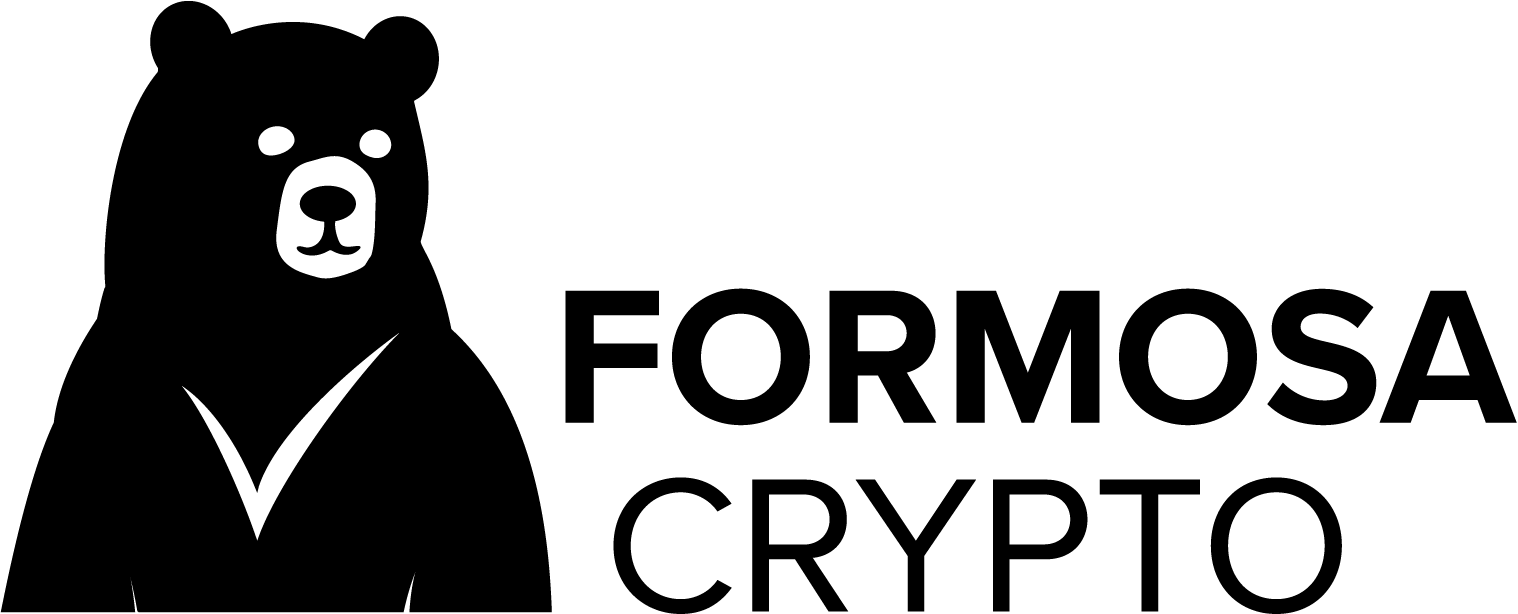
\includegraphics[width=0.4\textwidth]{formosa}
      \caption*{\Large \url{formosa-crypto.org}}
    \end{figure}
  \end{center}
  \vspace*{.5cm}
  \begin{itemize}
  \item[] \textbf{Jasmin:} \url{github.com/jasmin-lang/jasmin}
  \item[] \textbf{EasyCrypt specifications:}
    \url{github.com/formosa-crypto/crypto-specs}
  \item[] \textbf{Libjade:} \url{github.com/formosa-crypto/libjade}
  \end{itemize}
\end{frame}


\end{document}
